\chapter[Conclusão dos Resultados]{Conclusão dos Resultados}

Apos a análise dos resultados finais dos questionários aplicados, for possível rastrear a evolução da usabilidade entre as versões dos protótipos em relação à aplicação final, mesmo com o número de entrevistados tenha sido menor ao longo dos testes. Com base nas médias das respostas destes formulários, ficou evidente que houve uma melhora na experiência do usuário, apesar de que a maioria dos entrevistados não ter notado a diminuição do escopo durante a aplicação dos testes com o protótipo. Portanto, concluímos que as metas pré definidas a serem atingidas pela nossa aplicação foram cumpridas, dado que as perguntas foram definidas com base nestas metas, e como foi citado anteriormente, todas as perguntas estavam na forma de afirmações sobre o nosso site.

	O resultado final de nossa aplicação pode ser visto na figura abaixo.
	
\begin{figure}[H]
	\begin{center}
		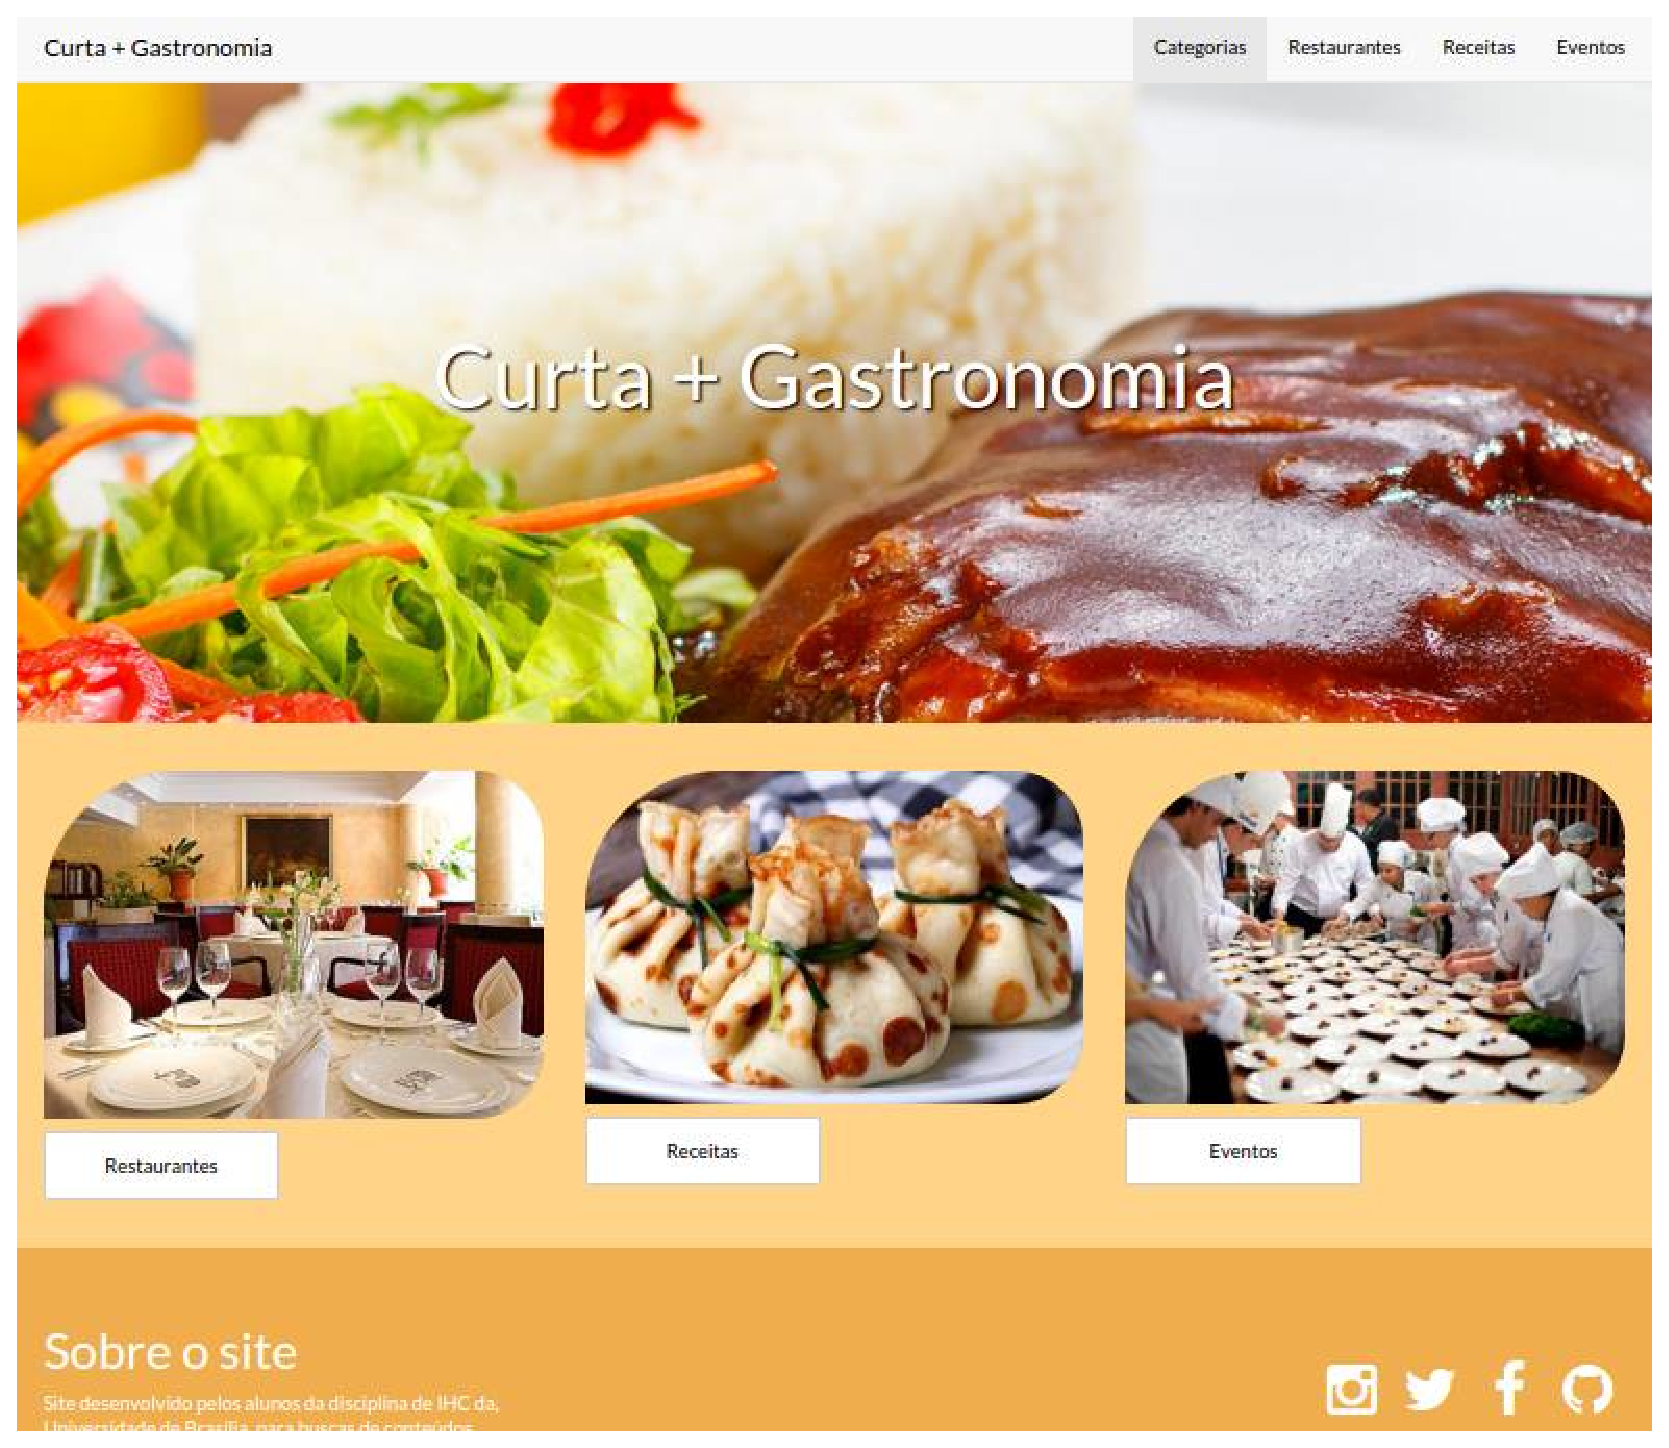
\includegraphics[keepaspectratio,scale=0.5]{figuras/aplicacao_final.eps}
		\caption{Website Versão Final: Curta Mais - Gastronomia}
	\end{center}
\end{figure}